%!TEX root = Lefley - Mesh to voxel transformations for optimised physics-based interactions.tex
\chapter{Implementation}

This chapter will discuss the stages of development. The starting point, implementation and result of each pipeline stage will be detailed as well as any difficulties faced.

\section{Process}

The process for development was iterative, implementing each pipeline stage in order. This was because each stage required the output of the previous stage to function and, while mock results could have been generated and forwarded, often the easiest way to input interesting data was to generate it from the previous stage because of the size of the data structures being used.

Stages were kept as encapsulated as possible so that any changes that had to be made would not cascade through later stages or require changes to those previous.

Testing and debugging were done on each stage as it was completed to test the performance of that particular implementation and gauge whether changes or a new algorithm were needed. This also improved the ease of finding bugs in comparison with debugging at the end of the pipeline.

\section{Preprocessing}

\label{sect:pre}

The simplest way to satisfy the requirement of applying the correct resultant movement vector to each fragment is to perform the fragmentation before the collision takes place. This allows the Unity3D physics engine to properly apply force to each fragment when the incoming particle makes contact.

It is therefore necessary to predict and extrapolate possible collisions before they occur. This was achieved by adding a bounding sphere to destructible objects and using Algorithm~\ref{alg:extrap}.

\begin{algorithm}[H]
 \KwData{Object to be destroyed: d, Bounding sphere: s, Incoming object: p}
 \KwResult{Force magnitude exerted on each object: f, Collision point on d: c}
 Ray r = cast ray from p along p.velocity\;
 \If{r intersects d}{
 	Point c = intersection point\;
 	Vector n = c.normal\;
 	n = n*2\;

 	Double md = d.mass\;
 	Double mp = p.mass\;

 	Vector vd = d.velocity\;
 	Vector vp = p.velocity\;

 	Double t = Physics.timestep\;

 	f = Dot(n, (mpvd - mdvp))\;
 	f = f / (md+mp)\;
 }
 \caption{Collision extrapolation}
 \label{alg:extrap}
\end{algorithm}

This algorithm relies on the following equations which approximately calculate the magnitude of the force which will be exerted on each object\footnote{Dylan Kennedy, personal communication, January 14, 2015}:

\begin{equation}
F = {\beta \over t} \quad \text{$t$ = time objects are in contact for}
\end{equation}

\begin{equation}
\beta = {2\mathbf{\hat{N_1}}\cdot (m_{2}\mathbf{v_1}-m_{1}\mathbf{v_2}) \over m_{1}+m_{2}}
\end{equation}

As the colliding objects are rigid we take the time that they will be in contact for to be one time-step of the Unity3D physics engine.

\subsection{Assumptions}

As we are extrapolating the collision data at the point when they enter the bounding sphere, some assumptions are made.

\begin{itemize}
\item{The velocity of the two objects involved will not change between this point and any collision}
\item{A third object will not move to obstruct any collision after this point}
\item{The rotation of either object will not change the result of any collision}
\end{itemize}

By tightening the bounding sphere around our destructible object we can take these assumptions to hold for simplicity.

\section{Voxelisation}

Originally it was planned for only a portion of the destructible object to be voxelised, depending on the physical forces involved. However it was found that the computational complexity of determining which mesh triangles fell within this portion was equal to that of voxelising these triangles. Therefore, for simplicity, the whole mesh is voxelised.

The solution for voxelisation used is based on an implementation of the Schwartz method found in GPU Pro 3\cite{Schwarz:2010:Vox}\cite{Engel:2012:GPA:2331213}.

This method is made up of two phases, a triangle phase and a propagation phase. Both of these are separate shaders run on the GPU to allow for parallel processing within the phases.

\subsection{Data structures}

The data structures used in this stage of the pipeline are primarily buffers as these can be passed to and from the GPU shaders as input and output.

The inputs to the first shader are the triangles defining the object's mesh. These are stored in two buffers. A `vertex' buffer stores a list of floating point numbers, each one being an x, y or z coordinate in a triangle's vertex, relative to the position of the object\footnote{Therefore the world position is not factored into the vertices.}. These values are always grouped such that for each vertex the x, y and z coordinates are adjacent and in sequence. There is no further ordering imposed. A second `index' buffer stores an integer list of indices into the vertex buffer. This buffer is ordered such that, when divided into strides of three, each index within that triplet refers to the point of a triangle when used with the vertex buffer. This is shown in Figure~\ref{fig:3.1}.

\begin{figure}
\centerline{\includegraphics[scale=0.5]{buffers13.pdf}}
\caption{The triangle (c) is represented by three consecutive indices, one for each vertex, in (b) which each point to the beginning of three consecutive floats which define that vertex in (a).}
\label{fig:3.1}
\end{figure}

The output from both shaders and input to the second is a three dimensional array of bits defining which voxels exist. This is stored as a single integer buffer, with each integer encoding 32 voxels. The three dimensional array is flattened, first along the $Z$ direction, then $X$, then $Y$. The $Z$ direction is padded such that all of the voxels in a integer will have the same $X$ and $Y$ coordinates. On being outputted from the second shader this flattened array is wrapped in a helper class which allows easy lookup into the array as if it were three dimensional as well as helper functions such as getting the array's size in any of the three dimensions represented.

%Figure?

\subsection{Triangle Phase}

During this phase, each triangle in the object to be voxelised is processed in its own GPU thread. First the triangle is translated and scaled by a pair of matrices defined by the object's bounding box and the requested voxel resolution\footnote{The $X$, $Y$ and $Z$ dimensions of the voxel grid.}. This transforms object relative world coordinates into `voxel coordinates'. 

The object relative coordinates are defined by taking a tight bounding box around the object, the centre of the box is $(0,0,0)$ and the box extends to $0.5$ in each dimension. Voxel coordinates define $(0,0,0)$ to be a corner of the bounding box and each axis extends to a defined magnitude depending on the voxel resolution desired. This is shown in Figure~\ref{fig:3.2}.

\begin{figure}
\centerline{\includegraphics[scale=0.5]{coordinates13.pdf}}
\caption{The box (a) represents a voxel space of resolution $7\times9\times7$. (b) shows the same box in object relative coordinates.}
\label{fig:3.2}
\end{figure}

Triangles are then projected onto the $XZ$ plane and all of the intersecting voxel columns are found\footnote{Voxel columns extending along the $Y$ axis.}. This is shown in Figure~\ref{fig:3.2.1}. For all of these columns the first voxel below the triangle, in the $Y$ direction, is set.

\begin{figure}
\centerline{\includegraphics[scale=0.5]{projection13.pdf}}
\caption{The red triangle has been projected onto the $XZ$ plane and the intersecting voxel columns marked in green.}
\label{fig:3.2.1}
\end{figure}

\subsection{Propagation Phase}

In the propagation phase we move up the $Y$ axis, XORing each voxel with the one below in the $Y$ direction. This allows us to fill in the solid volume. As we move up, when the first set voxel is met all those above will then become set until we reach another that had been set by the triangle phase. Each $Y$ column is processed in parallel, with 32 columns being processed in parallel on the same thread as we are XORing integers which are encoding 32 voxels.

\subsection{Progress}

\label{sect:voxprog}

Both shaders were taken from the GPU Pro 3 library mostly unaltered\footnote{There were methods in the first shader for other, unneeded, forms of voxelisation which were removed.}. The {\sc{C++}} driver found in the library was used to gain insight on interfacing with the shaders when writing the {\sc{C\#}} driver used. The completed driver and wrapper for the voxel grid output were heavily inspired by a {\sc{Javascript}} CPU implementation of voxelisation in Unity3D\cite{CPUVoxel}.

Achieving binary solid voxelisation on the GPU was the first major milestone completed. Several other libraries and methods were tried and tested before a suitable one was found. It also took much more time than anticipated to complete integration of the library which was used.

A scene was constructed where several objects differing in triangle resolution and shape were used for debugging the implementation. Figure~\ref{fig:3.3} demonstrates the output with the voxel structure being displayed for debugging.

\begin{figure}[b!]
\centerline{\includegraphics[scale=0.6]{Stanford_Bunny_Voxelised.png}}
\caption{Voxelisation of the `Stanford Bunny' model, composed of 69,666 triangles. The voxelisation shown is lower resolution than that which is typically used in the final implementation resulting in 1,723 voxels shown in red.}
\label{fig:3.3}
\end{figure}

\section{Physical Destruction}

\label{sect:destr}

The process of physically destroying an object involves partitioning its volume into fragments. This is done by assigning each voxel to a fragment, which will be referred to as `colouring'.

The method used is based on Voronoi diagrams as these are commonly used for achieving visually realistic fracturing effects\cite{Muller:2013:RTD:2461912.2461934}. This choice was made because of time restrictions and the encapsulated pipeline nature of Dynamic Volumetric Fragmentation would allow a more physically accurate algorithm to easily take its place.

\subsection{Data structures}

This pipeline stage takes the voxel grid from the voxelisation stage as an input and outputs a list of `fragment' classes and an altered voxel grid.

The fragment class stores:

\begin{itemize}
\item{An integer `colour' for that fragment, which acts as an identifier.}
\item{A list of points that make up the volume for that fragment.}
\item{A minimum and maximum $X$, $Y$ and $Z$ coordinate which define the bounding box for that fragment in voxel space.}
\end{itemize}

The altered voxel grid is a three dimensional array of integer values with each one corresponding to the colouring of the voxel in that position.

Duplicate information is returned here as different algorithms further down in the pipeline, primarily the meshing phase, require different input data structures. Some work on the point cloud provided by the fragment objects while others work optimally on the grid where neighbours can be found in constant time.

\subsection{Finding Generating Points}

To fragment the object using a Voronoi diagram, a series of generating points have to be found.

Firstly, the collision point from the preprocessing stage of the pipeline is transformed into voxel space. A number of vectors are then generated from this point with their magnitudes normally distributed within a given radius. The number of points and radius are calculated from both user defined physical properties of the object such as `brittleness' and `strength' as well as the collision force. This ensures that the fragmentation is different depending on the physical characteristics of the collision and therefore more accurate.

The vectors have normally distributed magnitudes so that there are more generating points closer to the collision point. This results in many smaller fragments about the point of impact as you would expect. 

\subsection{Partitioning}

Given the generating points $P_i$, a Voronoi diagram is a partitioning of space such that a cell contains all points in space which are closer to $P_i$ than any $P_j$. This is formally defined by equation~\ref{eq:3.1} and shown in Figure~\ref{fig:3.4}.

\begin{equation}
\text{Given a set } S=\{p_1, p_2\dotsc p_n\} \quad \text{A Cell } C(S,p_i)=\{p\in R^d\mid |p-p_i|<|p-p_j|, i\neq j\}
\label{eq:3.1}
\end{equation}

\begin{figure}
\centerline{\includegraphics[scale=0.25]{VoronoiEx.png}}
\caption{A Voronoi diagram\cite{voronoipict}.}
\label{fig:3.4}
\end{figure}

A fragment object is made for each generating point and all voxels are looped over. For each voxel, all generating points are checked and the closest found. That voxel is then added to the corresponding fragment object, also updating the minimum and maximum coordinates for that fragment, and the voxel is given the correct integer colouring in the new grid.

\subsection{Finding Islands}

\label{sect:islands}

A Voronoi partitioning is always guaranteed to produce convex solids when applied to a convex solid. However, as Dynamic Volumetric Fragmentation works on concave models this cannot be relied on. If a partitioning spans a concavity then it may produce unconnected islands as shown in Figure~\ref{fig:3.5}. Meshing such a partition into a rigid solid would result in floating areas as the physics engine cannot reason within a mesh as seen in Figure~\ref{fig:3.5.1}.

\begin{figure}
\centerline{\includegraphics[scale=0.5]{island13.pdf}}
\caption{The blue Voronoi cell creates two unconnected partitions of the concave object.}
\label{fig:3.5}
\end{figure}

\begin{figure}
\centerline{\includegraphics[scale=0.5]{islands.png}}
\caption{If the unconnected ears and body are a single mesh then the physics engine cannot act on the ears causing them to fall.}
\label{fig:3.5.1}
\end{figure}

To find and remove any islands a flood fill algorithm is used. Algorithms \ref{alg:flinit} and \ref{alg:flood} demonstrate how this works.

\begin{algorithm}[]
 \KwData{Dictionary of fragments indexed by colour: d, Greatest fragment colour: c, Coloured grid with islands: g}
 \KwResult{Dictionary of new fragments with no islands: o, Coloured grid with no islands: g}
 Dictionary$<$integer, fragment$>$ o\;
 \For{Each fragment f in d}{
 	\For{Each voxel v in f}{
 		\If{g[v.x,v.y,v.z] == f.colour}{
 			Fragment r\;
 			r.colour = ++c\;
 			o.Store(r.colour, r)\;
 			Flood(v.x, v.y, v.z, f.colour, r.colour, r, o)\;
 		}
 	}
 }
 \caption{Flood initiation}
 \label{alg:flinit}
\end{algorithm}

\begin{algorithm}[]
 \KwData{Vector to flood from: v, Old colouring: f, New colouring: r, Dictionary of fragments indexed by colour: o, Coloured grid with islands: g}
 \KwResult{Dictionary of new fragments with no islands: o, Coloured grid with no islands: g}
 Queue$<$Vector$>$ neighbours\;
 HashSet$<$Vector$>$ visited\;
 neighbours.Enqueue(v)\;
 visited.Add(v)\;
 \While{neighbours is nonempty}{
 	Vector deq = neighbours.Dequeue()\;

    int x = deq.x\;
    int y = deq.y\;
    int z = deq.z\;

    g[x, y, z] = r\;

    colouring.Add(v)\;

    \For{i from -1 to 1} {
        \For{j from -1 to 1} {
            \For{k from -1 to 1} {
                int xi = x + i\;
                int yj = y + j\;
                int zk = z + k\;

                \If{i == 0 AND j == 0 AND k == 0}{continue\;}
                \If{xi out of bounds in g OR yj out of bounds in g OR zk out of bounds in g}{continue\;}

                \If {g[xi, yj, zk] == f}{
                    \If{!(visited.Contains(xi, yj, zk))}{
                        neighbours.Enqueue(xi, yj, zk)\;
                        visited.Add(xi, yj, zk)\;
                    }
                }
            }
        }
    }
 }
 \caption{Flooding}
 \label{alg:flood}
\end{algorithm}

For every voxel in every fragment, if that voxel is still coloured with the same value as that fragment then it has not been reached by a previous flood for that fragment. Therefore it is not connected to the already flooded portion of that fragment and should instead be part of a new fragment. As should all connected voxels found by flooding from the voxel.

\subsection{Progress}

All of the code for this stage of the pipeline was written from scratch. Most time was spent optimising for both time and space complexity once the algorithms used had been implemented.

Debugging was done by partitioning the voxel structure of a cube and colouring the voxels according to their fragments. The generating points were also visualised. This is shown in Figure~\ref{fig:3.6}.

\begin{figure}[b!]
\centerline{\includegraphics[scale=1]{Voronoi.png}}
\caption{A visualisation of the Voronoi partitioning of the voxel structure of a cube.}
\label{fig:3.6}
\end{figure}

\subsection{Advantages}

As discussed, while the partitioning here is done using a Voronoi method which is common when working with surface representations, having a volumetric representation of an object could allow more complex and physically accurate algorithms. For example, the grid of voxels could be taken to represent the crystalline structure of some solids with the `bonds' between neighbouring voxels acting as they would in a real collision.

Also, the method works on both convex and concave models equally which is uncommon in other approaches as discussed in Section~\ref{sect:prob}.

\section{Intermediate Processing}

Before the partitioned voxels can become rigid meshes, preprocessing is needed. This is in order to prepare the data for the different algorithms used.

\subsection{Separating Border Voxels}

For the chosen meshing processes, the voxel grid is trimmed so that only interior border voxels remain, as shown in Figure~\ref{fig:3.7}. The reason for this is that both meshing processes require only the surface of the fragments defined by the voxels and not the solid volume. Separation is done by checking for every voxel whether it has a neighbouring voxel with a different colouring and keeping only those that do.

\begin{figure}[b!]
\centerline{\includegraphics[scale=0.9]{border213.pdf}}
\caption{A fragmented voxelised rectangle. The interior border voxels are green and the exterior voxels are blue. The unneeded interior voxels are red.}
\label{fig:3.7}
\end{figure}

Voxels on the surface of the object, with a non-existent neighbour, are recorded for entry into a k-d~tree.

A k-d tree is a binary tree based data structure which features an average $\mathcal{O}(n\log{}n)$ lookup for the nearest vector in the tree to a given vector in space.

An implementation of k-d trees in {\sc{C\#}} for Unity3D was found and used as there was little point reimplementing a well used data structure\cite{kdtree}.

Voxels both on the surface and on the interior borders with other fragments are also stored in the fragment they belong to.

\section{Mesh Generation}

Once the solid volume for each fragment has been found, it needs to be transformed into a rigid mesh for use in the physics engine. These meshes are constructed via two processes. The first splits the original object mesh and the second forms new meshes around the solid voxel structures.

\subsection{Data Structures}

The mesh partitioning procedure takes as an input the k-d tree of surface voxels from the intermediate processing stage as well as the original object mesh. The output is a list of fragment submeshes and for each one, a k-d tree of the vertices which make up the border of that submesh. These meshes will be referred to as the external meshes. This is shown in Figure~\ref{fig:3.8}.

\begin{figure}[b!]
\centerline{\includegraphics[scale=0.35]{mesh_border.png}}
\caption{A partitioning of the Stanford Bunny mesh. The vertices which make up the border of the green submesh are highlighted in red. The gap between partitions is caused by the loss of triangles which have vertices in different partitions.}
\label{fig:3.8}
\end{figure}

The marching tetrahedra algorithm runs for each fragment and takes as an input the grid of coloured border voxels from the intermediate processing stage as well as the k-d tree of the vertices which make up the fragment's external mesh border as outputted by the mesh partitioning procedure above. The algorithm outputs a mesh which represent the surface defined by the voxels (referred to as the solid mesh), and surface mesh, for that fragment.

\subsection{Mesh Partitioning}

\label{sect:part}

In order to preserve the original surface of the object the correct sections of the original mesh need to be mapped onto the computed fragments.

To do this the original object mesh is partitioned according to the colouring of the nearest voxel for every vertex.

This is the purpose of having all of the surface voxels in a k-d tree. There is no need to have the internal voxels as there will always be a surface voxel which is closer.

The process loops over all triangles and each vertex in that triangle. If all of the vertices have a nearest voxel of the same colouring then that triangle is added to the mesh for the fragment of that colouring. If the nearest voxel colours differ then the triangle is discarded and the vertices are added to the boundary k-d tree for their fragments.

The result of this process is demonstrated in Figure ~\ref{fig:3.8}. 

\subsection{Marching Tetrahedra}

\subsubsection{Marching Cubes}

Marching cubes is an algorithm used to extract a polygonal mesh of an implicit surface from a three-dimensional discrete scalar field\cite{Lorensen:1987:MCH:37401.37422}. The binary field of voxels\footnote{The colouring of the voxels is for identifying which fragment they belong to, they are still treated as binary present or not present for meshing purposes.} representing the solid volume of an object in this case is such an example.

The algorithm proceeds through the scalar field, taking a `cube' of eight adjacent locations at a time. The polygon(s) needed to represent the part of the implicit surface that passes through this cube are determined by creating an index into a pre-calculated array of 256 configurations from the eight scalar values.

Ordinarily each vertex of the generated polygons would be placed on the appropriate position along the cube's edge by linearly interpolating the two scalar values that are connected by that edge. However, in this case the scalar values only have two possibilities and so interpolating between them always results in a placement of the vertices half way between the voxels. This leads to a meshed surface which reveals the blocky voxel structure as opposed to a smoother surface which would be extracted if dealing with a field of actual scalars. This is shown in Figures \ref{fig:3.9} and \ref{fig:3.10}.

\begin{figure}[b!]
\centerline{\includegraphics[scale=8]{marchingtetrahedrons.jpg}}
\caption{Marching tetrahedra applied to a scalar field generated from perlin noise\cite{ScrawkMarching}.}
\label{fig:3.9}
\end{figure}
\begin{figure}
\centerline{\includegraphics[scale=0.75]{Marching.png}}
\caption{Marching tetrahedra applied to the voxel grid of a fragmented Stanford Bunny.}
\label{fig:3.10}
\end{figure}

Ambiguous cases are present in the polygonisation where there exist at least two correct interpretations of the implicit surface. This is shown in two dimensions\footnote{These ambiguities would therefore be for the marching squares algorithm but the premise is the same.} in Figure~\ref{fig:3.11}.

\begin{figure}
\centerline{\includegraphics[scale=0.5]{ambiguous.png}}
\caption{The two possible surfaces for the imaginary square shown with dashed lines with two points inside the surface and two outside.}
\label{fig:3.11}
\end{figure}

\clearpage
\subsubsection{Marching Tetrahedra}

Marching tetrahedra is an algorithm based on marching cubes which solves these ambiguities as well as producing a surface which matches the voxel data more closely at the cost of generating more vertices\cite{Tetrahedra}.

In marching tetrahedra, each cube is split into six irregular tetrahedra by cutting the cube in half diagonally three times as shown in Figure~\ref{fig:3.12}. These tetrahedra are then used to find the implicit surface in much the same way as marching cubes however there are now nineteen edge intersections per cube instead of twelve.

\begin{figure}[b!]
\centerline{\includegraphics[scale=0.8]{Marching_tetrahedrons.png}}
\caption{A cube split into six irregular tetrahedra\cite{marchingpict}.}
\label{fig:3.12}
\end{figure}

\clearpage
\subsubsection{Modification}

As two separate meshes are being produced in this stage, a section of the original mesh and a surface representing the solid volume, the two need to be combined and joined.

The marching tetrahedra library used was modified to take the grid of coloured border voxels as well as the set of voxels lying both on the exterior and on the fragment border. The k-d tree of the vertices which make up the fragment's external mesh border is also used. These border voxels are meshed using marching tetrahedra. However, when a voxel also lying on the exterior is found, the calculated vertices are discarded and instead their nearest neighbours in the k-d tree are used. This process knits the gap that would have otherwise existed between the two generated meshes, the external mesh and the solid mesh. A small amount of random noise is also applied to the rest of the vertices in an effort to disguise some of the blocky underlying structure. The results of this can be seen in Figure~\ref{fig:3.13}.

\begin{figure}
\centerline{\includegraphics[scale=0.75]{collision.png}}
\caption{The Stanford Bunny after the entire pipeline has completed.}
\label{fig:3.13}
\end{figure}

\subsection{Progress}

This stage of the pipeline took the longest to complete and was the final milestone when done. The stage went through several iterations of varying success before the above method was devised.

Originally the fragment meshes were to be only generated using marching tetrahedra with no splitting or use of the original external mesh. This resulted in an important detail loss as seen in Figure~\ref{fig:3.10} and was not viable for use. Increasing the voxel resolution improved this but added too much of a computational overhead.

A second method involved only splitting the original external mesh and not using marching tetrahedra at all. The resultant fragment meshes were duplicated and had their normals flipped before being combined. This gave results that resembled hollow porcelain objects as seen in Figure~\ref{fig:3.14}. This could not be used as it did not satisfy the requirement of modelling the internal structure.

\begin{figure}
\centerline{\includegraphics[scale=1]{Porcelain2.png}}
\caption{The Stanford Bunny fractured as if it were a hollow object.}
\label{fig:3.14}
\end{figure}

Producing the final method, involved modifying the marching cubes library found to stitch the external and solid meshes together as discussed. The algorithm found in the library was also optimised. Originally the algorithm would produce duplicate vertices for triangles which should share a vertex. This was solved by using a dictionary of vertices and indices into the vertex list. All vertices required by a triangle are checked in the dictionary, if they exist as a key then the index stored is used else the vertex is added to the vertex list and a new index stored in the dictionary with that vertex and used in the triangle. This dramatically reduced vertex counts in the meshes produced which is necessary as Unity3D imposes a limit of 65,534 vertices for any mesh.

\section{Post-processing}

After the fragment meshes have been generated, some post processing must take place in order for the meshes to be used in the physics simulation.

\subsection{Physics}

\label{sect:postphysics}

One advantage of fragmenting a voxel structure is that the mass of each fragment, $m_f$, can be calculated using Equation~\ref{eq:mass}.

\begin{equation}
\begin{split}
m_f=m_o\times v_f/v_o \quad \text{$v$ is the number of voxels}
\label{eq:mass}
\end{split}
\end{equation}

\subsection{Game-object Generation}

Finally, the fragment meshes and masses are passed to Unity3D so that they can be instantiated into the simulated world. Depending on the number of vertices in each mesh this can add a large time overhead which will be discussed in Section~\ref{sect:over}. This overhead is a limitation of Unity3D and not Dynamic Volumetric Fragmentation.

\section{Result}

\label{sect:result}

The result is a library which can be used to fragment objects on collision based on the physical attributes of the object and of the collision.

The library produced requires that two scripts be attached to the destructible object, one as a driver for the destruction process and the other to allow the physical properties of the object to be defined. A Unity3D object with a `sphere collider' must also be attached with a script which triggers the destruction process as detailed in Section~\ref{sect:pre}. All of these elements are added to an existing object and none require any existing features of the object to be changed.

When an object is given the above attributes and a projectile fired at it, the object is broken into fragments and these fragments then receive force from the projectile causing them to explode out as would be expected. This is shown in Figure~\ref{fig:3.15}.

A video demonstrating the results can be found at \url{https://www.screenr.com/NRQN}.

\begin{figure}
\centerline{\includegraphics[scale=0.7]{voxel_exploded.png}\includegraphics[scale=0.686]{voxel_exploded2.png}}
\caption{Fragments exploding out of the Stanford Bunny after a cubic projectile, shown in red, has been fired at it.}
\label{fig:3.15}
\end{figure}

The nature of the fragmentation differs depending on the forces involved as shown in Figure~\ref{fig:3.16}.

\begin{figure}
\centerline{\includegraphics[scale=0.85]{voxel_forces.png}}
\caption{The biggest fragments after three Stanford Bunnies have been fragmented. Compared to the middle, the right was given a higher strength while the left was hit with a faster projectile.}
\label{fig:3.16}
\end{figure}

\section{Conclusion}

In order for the proposed solution to be realised, four stages of implementation had to take place:

\begin{enumerate}
\item{Preprocessing}
\label{point:pre}
\item{Voxelisation}
\label{point:vox}
\item{Meshing}
\label{point:mesh}
\item{Postprocessing}
\label{point:post}
\end{enumerate}

Intermediate stages were also completed to process data passed between the above sections.

Points \ref{point:vox} and \ref{point:mesh} required adapting existing implementations of the algorithms used whereas the remaining sections were developed from scratch.